%\documentclass[letterpaper, 12pt, openany]{book}
\documentclass[openany]{report}
\usepackage[utf8]{inputenc}
\usepackage[spanish]{babel}
\usepackage{cite,url,graphicx,amsmath,amssymb,enumitem,amsthm,appendix}
%\usepackage{fullpage}
\usepackage{authblk}
%bibliografia
%\usepackage{babelbib}
%\selectbiblanguage{spanish}
%\usepackage{csquotes}
%\usepackage[sorting=nyt,style=apa,backend=biber]{biblatex}

%dimensiones oficiales
\usepackage[paperwidth=17cm,paperheight=22.5cm,margin=2cm]{geometry}
%para revision ("frame" para cuadrito)
\usepackage[letter,center,noinfo]{crop}

%para definir bibliografia en referencias
%\usepackage{etoolbox}
%\makeatletter
%\renewcommand{•}{•}\baselinestretch}{1.5}

% Para algoritmos (Gracias Andreu)
%\usepackage[ruled,lined,boxed,linesnumbered,spanish]{algorithm2e}
%\SetKwInput{Input}{Entrada}
%\SetKwInput{Output}{Salida}
%\SetKwIF{If}{ElseIf}{Else}{si}{entonces}{de otro modo si}{de otro modo}{fin del si}
%\SetKwFor{For}{para}{hacer}{fin del para}
%\SetKwFor{While}{mientras}{h
%\patchcmd{\thebibliography}{%
%  \chapter*{\bibname}\@mkboth{\MakeUppercase\bibname}{\MakeUppercase\bibname}}{%
%  \chapter*{Bibliografía}}{}{}
%\makeatother

%definición de definicones matemágicas
\newtheorem{defn}{Definición}

%espacio entre párrafos
%\setlength{\parskip}{6pt}

%interlineadoacer}{fin}
%\SetKwRepeat{Do}{hacer}{mientras}

\usepackage{algorithm}
\usepackage{algpseudocode}
\renewcommand{\algorithmicrequire}{\textbf{Entrada:}}
\renewcommand{\algorithmicensure}{\textbf{Salida:}}


\title{Estudio de algoritmos de planificación para flujos de trabajo}
\author{Fernando Aguilar Reyes}

\affil{Tesis para obtener el título de Ingeniero en Computación \\
       Instituto Tecnológico Autónomo de México \\
     Río Hondo 1, Progreso Tizapán, Del. Álvaro Obregón, 01080 \\
     México, Distrito Federal \\}

\begin{document}

\maketitle

\tableofcontents

\listoffigures
	
%\mainmatter
\chapter{Introducción}
Cada día, los cómputos son más complejos. Hay bancos que procesan millones de transacciones diarias. Las películas de animación requieren vastos tiempos de cómputo. Muchos proyectos de computación científica requieren hacer numerosos cálculos para llegar a resultados pertinentes. ¿Qué tienen en común todas estas aplicaciones? Ya hemos mencionado que toman mucho tiempo en calcularse. Entonces, una posible solución para disminuir el tiempo de ejecución de estas aplicaciones es distribuir el gran trabajo que requieren estos proyectos entre varias computadoras. Para ello, necesitamos dividir nuestra aplicación en partes más pequeñas e independientes, algunas de ellas podrán ejecutarse de manera concurrente, otras no. De esta forma, tendríamos una solución escalable, es decir, si aumentamos el número de computadoras disponibles para nuestra aplicación, reduciremos el tiempo de ejecución.

Lograr esta paralelización requiere un esfuerzo por parte del desarrollador de la solución. Existen técnicas de paralelización que permiten al desarrollador expresar su programa en varias partes paralelas, por ejemplo: la administración multiproceso de los sistemas operativos, los threads en un proceso, el modelo MapReduce implementado en Hadoop, MPI implementado en OpenMPI. Aunque estas técnicas de paralelización son muy efectivas, éstas son aplicadas cuando el problema a resolver ha sido bien definido y cuando sólo hay una instancia del problema. Ahora bien, cuando la solución involucra varios pasos que están relacionados entre sí —por ejemplo, que el programa C requiera de la salida del programa A y del programa B para que pueda funcionar—, o cuando estamos definiendo los grandes bloques de solución del problema, hay una cierta secuencia que debemos seguir y, dentro de dicha secuencia, hay algunos pasos que podemos resolver de manera concurrente. Por lo tanto, estamos haciendo un \emph{modelo} de nuestro problema.

Este modelo también es llamado \emph{flujo de trabajo}. De manera muy abstracta, un flujo de trabajo es un conjunto de pasos que modelan la ejecución de un proceso. Este concepto ha sido aplicado en numerosas áreas. En el ámbito de los negocios, se utiliza diagramas dibujados con los bloques y reglas del \emph{Bussiness Process Execution Language} para modelar procesos de negocio.

En el ámbito de las ciencias en computación, los flujos de trabajo son aplicados para modelar problemas que requieran varios pasos para su solución. Algunos flujos de trabajo requieren mucho tiempo tiempo de ejecución para sus pasos, como son el caso de los flujos de trabajo científicos. Otros flujos de trabajo son muy simples pero  se requieren que se ejecuten muchos de éstos. De esta forma, es desable distribuir la ejecución de éstos flujos de trabajo entre varias computadoras. Si bien es posible paralelizar algunos pasos de la ejecución de nuestro flujo de trabajo utilizando las técnicas antes mencionadas, hay restricciones de orden que se deben respetar, por lo cual, se debe planear la ejecución del flujo de trabajo.

Hay varias maneras de hacer esta planeación de la ejecución, también llamada \emph{calendarización}. Cabe aclarar que definimos la calendarización como la asignación de recursos a tareas de tal modo que se ejecuten todas las tareas. Con ello, se desea encontrar una forma óptima de hacer esta calendarización, como reducir el tiempo de ejecución total del flujo de trabajo. Sin embargo, con la aparición del cómputo en la nube, es posible ejecutar nuestro flujo de trabajo con otras restricciones, como minimizar el presupuesto necesario para la ejecución del flujo afectando el tiempo de ejecución.

%mencionar instruction level paralelism, task level paralelism, 

%uml, bepl para software y negocios, buscar los que vienen en el paper de hierarchical scheduling for swindew-c

En esta tesina se hace un estudio de los principales algoritmos de calendarización de flujos de trabajo, con énfasis en los algoritimos utilizados en cómputo distribuido, en especial en cómputo en la nube. En el capítulo 2 se habla de un estudio detallado del concepto de flujos de trabajo y su aplicación en computación. El capítulo 3 trata los principales enfoques de cómputo distribuido para ejecutar estos flujos. En el capítulo 4 se hace un estudio de los principales algoritmos de calendarización de los flujos. Finalmente, en el capítulo 6 discutiremos algunas conclusiones sobre el análisis de estos algoritmos.

\chapter{Flujos de trabajo}
\label{chap:workflows}

\section{Definición y ejemplos}
Un flujo de trabajo es un conjunto de pasos que modelan la ejecución de un proceso \cite{gutierrez2012agent}.
%En la literatura especializada, los flujos de trabajos también son conocidos como \emph{workflows}.%
En particular, en esta tesis se estudian a los flujos de trabajo utilizados para vislumbrar la ejecución de un proceso de cómputo. A continuación, se muestran algunos ejemplos de estos flujos de trabajo.

\subsection{Anotación de proteínas}
En el proyecto \emph{e-Protein}, realizado por la Escuela Imperial de Londres, se realizó un flujo de trabajo para la anotación de proteínas. El objetivo del proyecto \cite{o2004mapping} era la identificación y anotación de partes de proteínas que expliquen su estructura y su función. En la figura \ref{fig:iceni-workflow} se muestra el flujo de trabajo desarrollado, donde las cajas representan los programas que son ejecutados para cada paso del proceso de anotación, y las líneas que conectan a las cajas representan las dependencias de datos entre los programas, es decir, si una caja tiene una línea que apunta a ella, significa que dicho programa depende de otro porgrama determinado por el otro extremo de la flecha.

\begin{figure}
    \begin{center}
        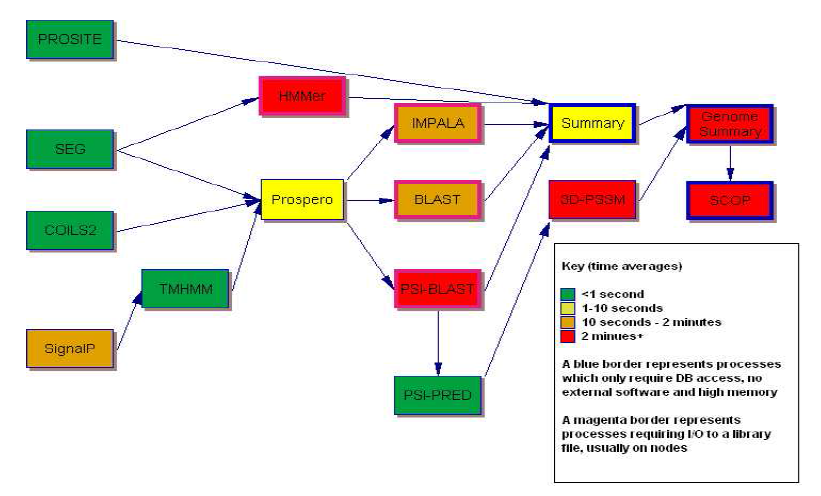
\includegraphics[width=0.8\textwidth]{imagenes/iceni-workflow}
    \end{center}
    \caption{Flujo de trabajo para la anotación de proteínas.}
    %diseñado en la Escuela Imperial de Londres para el proyecto \emph{e-Protein}.
    \label{fig:iceni-workflow}
\end{figure}


\subsection{Curvas de amenaza sísmica}
Otro notable ejemplo es el proceso para generar curvas de amenaza sísmica que describen las probabilidades de que ocurra un temblor en una determinada área. Para elaborar estas curvas, los científicos del Centro de Terremotos del Sur de California (SCEC por sus siglas en inglés) tienen que realizar una gran cantidad de simulaciones para que sus resultados puedan ser combinados y expresados en la curva de amenaza \cite{deelman2006managing}. El flujo de trabajo para generar la curva de amenaza se muestra en la figura \ref{fig:scec-workflow}.

\begin{figure}
    \begin{center}
        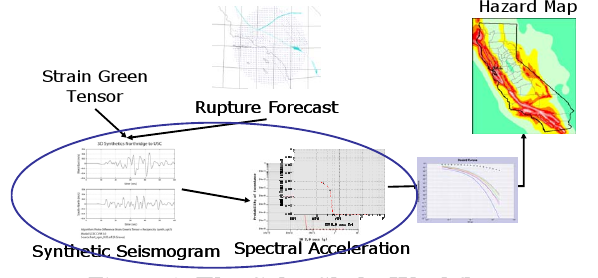
\includegraphics[width=0.8\textwidth]{imagenes/scec-workflow}
    \end{center}
    \caption{Flujo de trabajo para generar curvas de amenaza sísmica.}
    %elaborado por el SCEC
    \label{fig:scec-workflow}
\end{figure}

\subsection{Generación de facturas}
Recientemente en México, el Sistema de Administración Tributaria emitió los lineamientos para que las operaciones de compra-venta entre personas físicas y morales puedan ser registradas por medio de facturas electrónicas. Para generar estos Comprobantes Fiscales Digitales, las empresas tienen que hacer procesos de validaciones de RFC y encriptar el contenido de la factura con un mecanismo de llave privada. Naturalmente, este proceso de generación de factura requiere de varias actividades. En la figura \ref{fig:cfd-workflow} se muestra el flujo de trabajo que utiliza una empresa para generar sus facturas. Este flujo se encuentra documentado en una tesina presentada por Alcerreca \cite{alcerreca2013cfd}.

\begin{figure}
    \begin{center}
        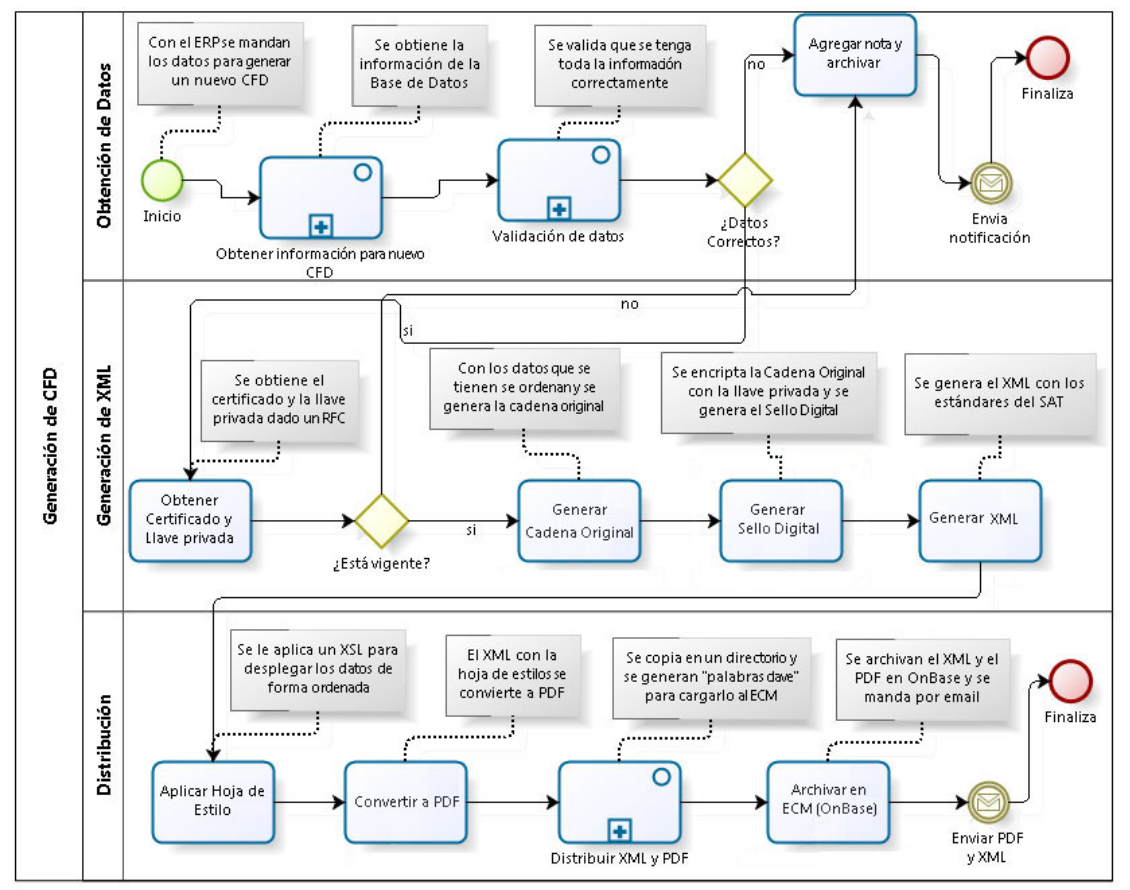
\includegraphics[width=0.8\textwidth]{imagenes/cfd-workflow}
    \end{center}
    \caption{Flujo de trabajo para generar facturas electrónicas.}
    %utilizado por una empresa de cementos
    \label{fig:cfd-workflow}
\end{figure}

\subsection{Procesamiento de imágenes astronómicas}

La NASA elaboró un software que permite crear una gran imagen del espacio exterior a partir de varias imágenes mosaico tomadas desde distintos telescopios. Esta aplicación, llamada Montage, utiliza un flujo de trabajo para generar la gran imagen. En la fase inicial de procesamiento, cada una de las imágenes mosaico puede ser procesada de manera independiente. En la figura \ref{fig:montage-workflow} se puede observar que el flujo de trabajo del proyecto Montage inicia con varias actividades en paralelo, donde el color de las actividades representan la fase de procesamiento de la imagen. Luego, en la acividad de color gris, todas las imágenes son juntadas para generar la imagen de fondo común para todas las imágenes mosaico.

\begin{figure}
    \begin{center}
        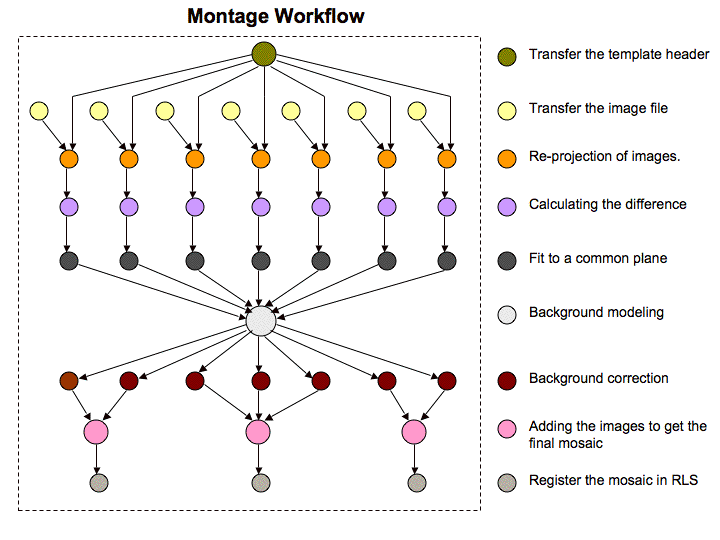
\includegraphics[width=0.8\textwidth]{imagenes/montage-workflow}
    \end{center}
    \caption{Flujo de trabajo para procesamiento de imágenes del proyecto Montage.}
    %utilizado por una empresa de cementos
    \label{fig:montage-workflow}
\end{figure}



\section{Estructura de los flujos de trabajo}
\label{secc:workflow_str}
Como hemos visto en los tres ejemplos anteriores, los flujos de trabajo presentados describen los \emph{pasos} que se necesitan para calcular la solución de un problema. En éstos, no se ha hablado sobre los detalles para hacer los cómputos necesarios para cada flujo. En los flujos de trabajo tampoco se han definido las plataformas de cómputo en que se ejecutan estos flujos. Tan sólo se han definido los grandes pasos para solucionar el problema y las dependencias que tienen estos pasos. 

Ahora, es muy común que estas dependencias estén dictadas por los datos que requiere cada paso para funcionar. Sin embargo, hay situaciones en los que los pasos del flujo no requieren los datos del paso anterior para funcionar, sino que las dependencias están marcadas por el orden temporal que deben seguir estos pasos. Así, se puede notar una ambigüedad en la definición de un flujo de trabajo.

\section{Perspectivas de los flujos de trabajo}
En la sección \ref{secc:workflow_str} se argumentó que un flujo de trabajo puede representar varias cosas, a saber: el orden temporal de las tareas o las dependencias de datos entre cada tarea, produciendo una ambigüedad en la interpretación de un flujo de trabajo. Debido a esta ambigüedad del significado de un flujo de trabajo, es posible interpretar un flujo de trabajo desde varias perspectivas. En el trabajo de Van der Aalst et al. \cite{van2003workflow} se identifican una serie de perspectivas identificadas en las definiciones de las especificaciones de un flujo de trabajo utilizadas en los sistemas que administran la ejecución de flujos de trabajo. Las cuatro perspectivas se enuncian a continuación:
%En esta tesis, tomaremos estas perspectivas a manera de una clasificación de flujos de trabajo basadas en la forma en que describen sus dependencias

\begin{itemize}
\item{\textbf{Perspectiva de control de flujo.} Describe las relaciones de las actividades (pasos) con estructuras de control, tales como: secuencia, decisión, ejecución de actividades en paralelo y punto de sincronización conjunta. El flujo de trabajo para la generación de facturas es un buen ejemplo de un flujo de trabajo visto desde la perspectiva de control de flujo porque, al observar la figura \ref{fig:cfd-workflow}, se pueden notar que hay actividades, simbolizadas con un rombo, que determinan si se ejecutan o no ciertas tareas.
%\footnote{Esta estructura de control también es conocida como \emph{join synchronization}}.
}

\item{\textbf{Perspectiva de datos.} En ella, los flujos de trabajo describen las entradas y salidas de datos, tanto de ejecución como de control, que se tienen en cada actividad del flujo. También se toman en cuenta los datos locales a cada actividad; es decir, que sólo son necesarios dentro del contexto de ésta. En el ejemplo del flujo de trabajo para la anotación de proteínas, mostrado en la figura \ref{fig:iceni-workflow}, podemos ver que esta perspectiva describe adecuadamente la estructura del flujo, ya que el orden de ejecución de las actividades están definidas por los datos que requiren cada una de las actividades.}

\item{\textbf{Perspectiva de recursos.} Muestra cuáles son los recursos con los que se cuentan para ejecutar el flujo de trabajo y la forma en que estos recursos se encuentran organizados. Estos recursos pueden ser desde entidades de cómputo hasta roles con responsabilidades específicas cumplidas por actores humanos. El flujo de trabajo para generar curvas de amenaza sísmica de la figura \ref{fig:scec-workflow} es un ejemplo de esta perspectiva, porque los elemenos necesarios para generar las curvas de amenaza son provistos por geólogos.}

\item{\textbf{Perspectiva operacional.} Aquí se detallan las operaciones elementales necesarias en cada actividad para ejecutar el flujo de trabajo. Estos detalles incluyen las transferencias de datos entre las operaciones y su correspondencia en programas. El flujo de trabajo del proyecto Montage, mostrado en la figura \ref{fig:montage-workflow} ejemplifica esta perspectiva, ya que los colores utilizados en el flujo de trabajo son las actividades específicas que se aplican a cada imagen a procesar.}
\end{itemize}

Cabe aclarar que estas perspectivas están relacionadas entre sí de modo que el control de flujo es la base en la que descansan las demás perspectivas. Esto es porque la perspectiva de datos requiere que el control de flujo tenga los datos de entrada y salida como prueba de que se cumplieron las pre y post-condiciones de cada actividad, respectivamente; la perspectiva de recursos define con qué se ejecutarán y almacenarán los datos del flujo de trabajo; mientras que la perspectiva operacional trata los detalles sobre cómo se utilizan físicamente los recursos, los datos y los programas a lo largo del flujo de trabajo.


\section{Planificación como control de flujo}

El hecho de que la perspectiva de control de flujo sea la base de las demás perspectivas indica que la forma en que controla la ejecución del flujo determina de manera fundamental el rendimiento de la ejecución total de una instancia del flujo de trabajo. Por lo tanto, es de vital importancia encontrar métodos de planificación que permitan encontrar correspondencias entre recursos y actividades que cumplan con los requisitos dictados en las especificaciones examinadas en la perspectiva del control del flujo y que también maximicen el rendimiento de la ejecución de todo el flujo en general.

\section{Alcance}

En este trabajo, se establecerán las siguientes consideraciones para definir el alcance de este estudio de los algoritmos de planificación, a saber: la utilización de grafos dirigidos acíclicos y la suposición de que no habrá errores en la ejecución atómica de las tareas de los flujos de trabajo. En las siguientes se explicarán la importancia de estas suposiciones.

\subsection{Grafos dirigidos acíclicos}
Los flujos de trabajo están representados como \emph{grafos dirigidos acíclicos}, con el objetivo de simplificar el estudio. Se utilizan estos grafos porque son una estructura de datos que representa intuitivamente las dependencias entre tareas. Se requiere que estos grafos sean dirigidos porque esta característica representa el orden de ejecución de las tareas. Además, el hecho de que no existan ciclos en los grafos implica que no se necesita ningún mecanismo de control de flujo condicional; es decir, si la ejecución de las tareas de un flujo de trabajo dependiera de las salidas de otras tareas del flujo, no se podría saber apriori cuál es el orden de ejecución de las tareas, y los algoritmos de planificacíón tendrían que especular cuál sería el posible orden de ejecución.

\subsection{Ejecución atómica de tareas sin fallos}
Las tareas (o actividades) de los flujos de trabajo son consideradas \emph{atómicas}, i.e., una tarea no puede ejecutarse incompletamente ni incorrectamente. Algunos sistemas de administración de ejecución de flujos de trabajo tienen mecanismos para lidiar con estos errores, pero el estudio de éstos queda fuera del alcance de este trabajo, debido a la complejidad que representa diseñar e implementar sistemas distribuidos tolerantes a fallos. Un ejemplo de un sistema de administración de flujos de trabajo se encuentra en el trabajo de Kandaswamy et al. \cite{kandaswamy2008fault}, en el cual describe que utilizan sobreprovisionamiento de recursos y migración de recursos para mitigar las fallas.

%\item{La información de las \emph{demás perspectivas} puede ser requerida, dependiendo si el mecanismo de planificación lo considere necesario para tomar mejores decisiones con el fin de optimizar el tiempo total de ejecución o cumplir con algunos criterios establecidos en la definición del flujo de trabajo.}

%conclusiones:
% - representar como DAG's porque es sencillo y expresivo (balanceado)
% - tareas atómicas
% - la información de las demás perspectivas se puede requerir o no, dependiendo de como lo requiera el planificador.


%ejemplo: ICENI tiene partes paralelas, que no requieren de ciertos datos para operar
%ejemplo: Si hablas de orden,
%poner ejemplos donse se ejemplifique esta calendarización

%clasificados de acuerdo a dependencias (de orden, o de datos)


%clasificados de acuerdo a nivel de detalle (específico para cada plataforma)

%clasificados de acuerdo a instancias
% - pocas instancias, mucho tiempo de cómputo:
% - intensivos en instancias, pero cortos en ejecución:

%todos se pueden representar como Grafos Dirigidos Acíclicos

%implementaciones de representación de workflows
% - AGWL
\chapter{Cómputo distribuido}
Los flujos de trabajo requieren de recursos de cómputo para su ejecución. En los flujos de trabajo de ejemplo del capítulo \ref{chap:workflows} se mencionaron aplicaciones científicas que, por su naturaleza, requieren un alto poder de cómputo para llevarse a cabo. Por otro lado, también existen aplicaciones de negocio que, si bien son computacionalmente sencillas, se requiere ejecutar una gran cantidad de instancias de estos flujos de trabajo. Por ello, ejecutar cualquiera de estos flujos de trabajo en una sola computadora resulta prohibitivo. Por lo tanto, comúnmente se hace uso de varias computadoras para distribuir la carga computacional necesaria para correr estos procesos.

Dependiendo de cómo estén organizados estas computadoras, se definen los enfoques para correr los flujos de trabajo con cómputo distribuido.

\section{Enfoques de cómputo para flujos de trabajo}
Diversos enfoques se han aplicado para distribuir la ejecución de un flujo de trabajo entre varias computadoras.  De acuerdo a Buyya et al., los enfoques de cómputo más importantes para los flujos de trabajo son los \emph{clusters}, los \emph{grids} y las \emph{nubes} \cite{buyya2009cloud}. A continuación, explicaremos cada uno de los enfoques.

\subsection{Clusters}
Los \emph{clusters} son sistemas distribuidos, paralelos, compuestos de varias computadoras conectadas entre sí que funcionan como un único recurso de cómputo \cite{buyya2009cloud}. 

Un ejemplo de un cluster se puede encontrar en la Universidad Autónoma Metropolitana, campus Iztapalapa. El cluster, llamado \emph{Aitzaloa}, está compuesto por 270 nodos de cómputo, cada uno equipado con dos procesadores Intel Xeon Quad-Core y 16GB en RAM; los nodos están conectados entre sí por medio de switches Ethernet e Infiniband. El cluster también cuenta con un sistema de archivos distribuido basado en Lustre. La capacidad real de cómputo del cluster Aitzaloa es de 18.4 teraFLOPS \cite{uamz2013tizaloa}.

El detalle de la topología del cluster se puede apreciar en la figura \ref{fig:topologia_aitzaloa}, en donde podemos apreciar que los switches son los puntos de conexión entre el nodo maestro, el sistema de almacenamiento distribuido y los nodos de cómputo.

\begin{figure}
    \begin{center}
        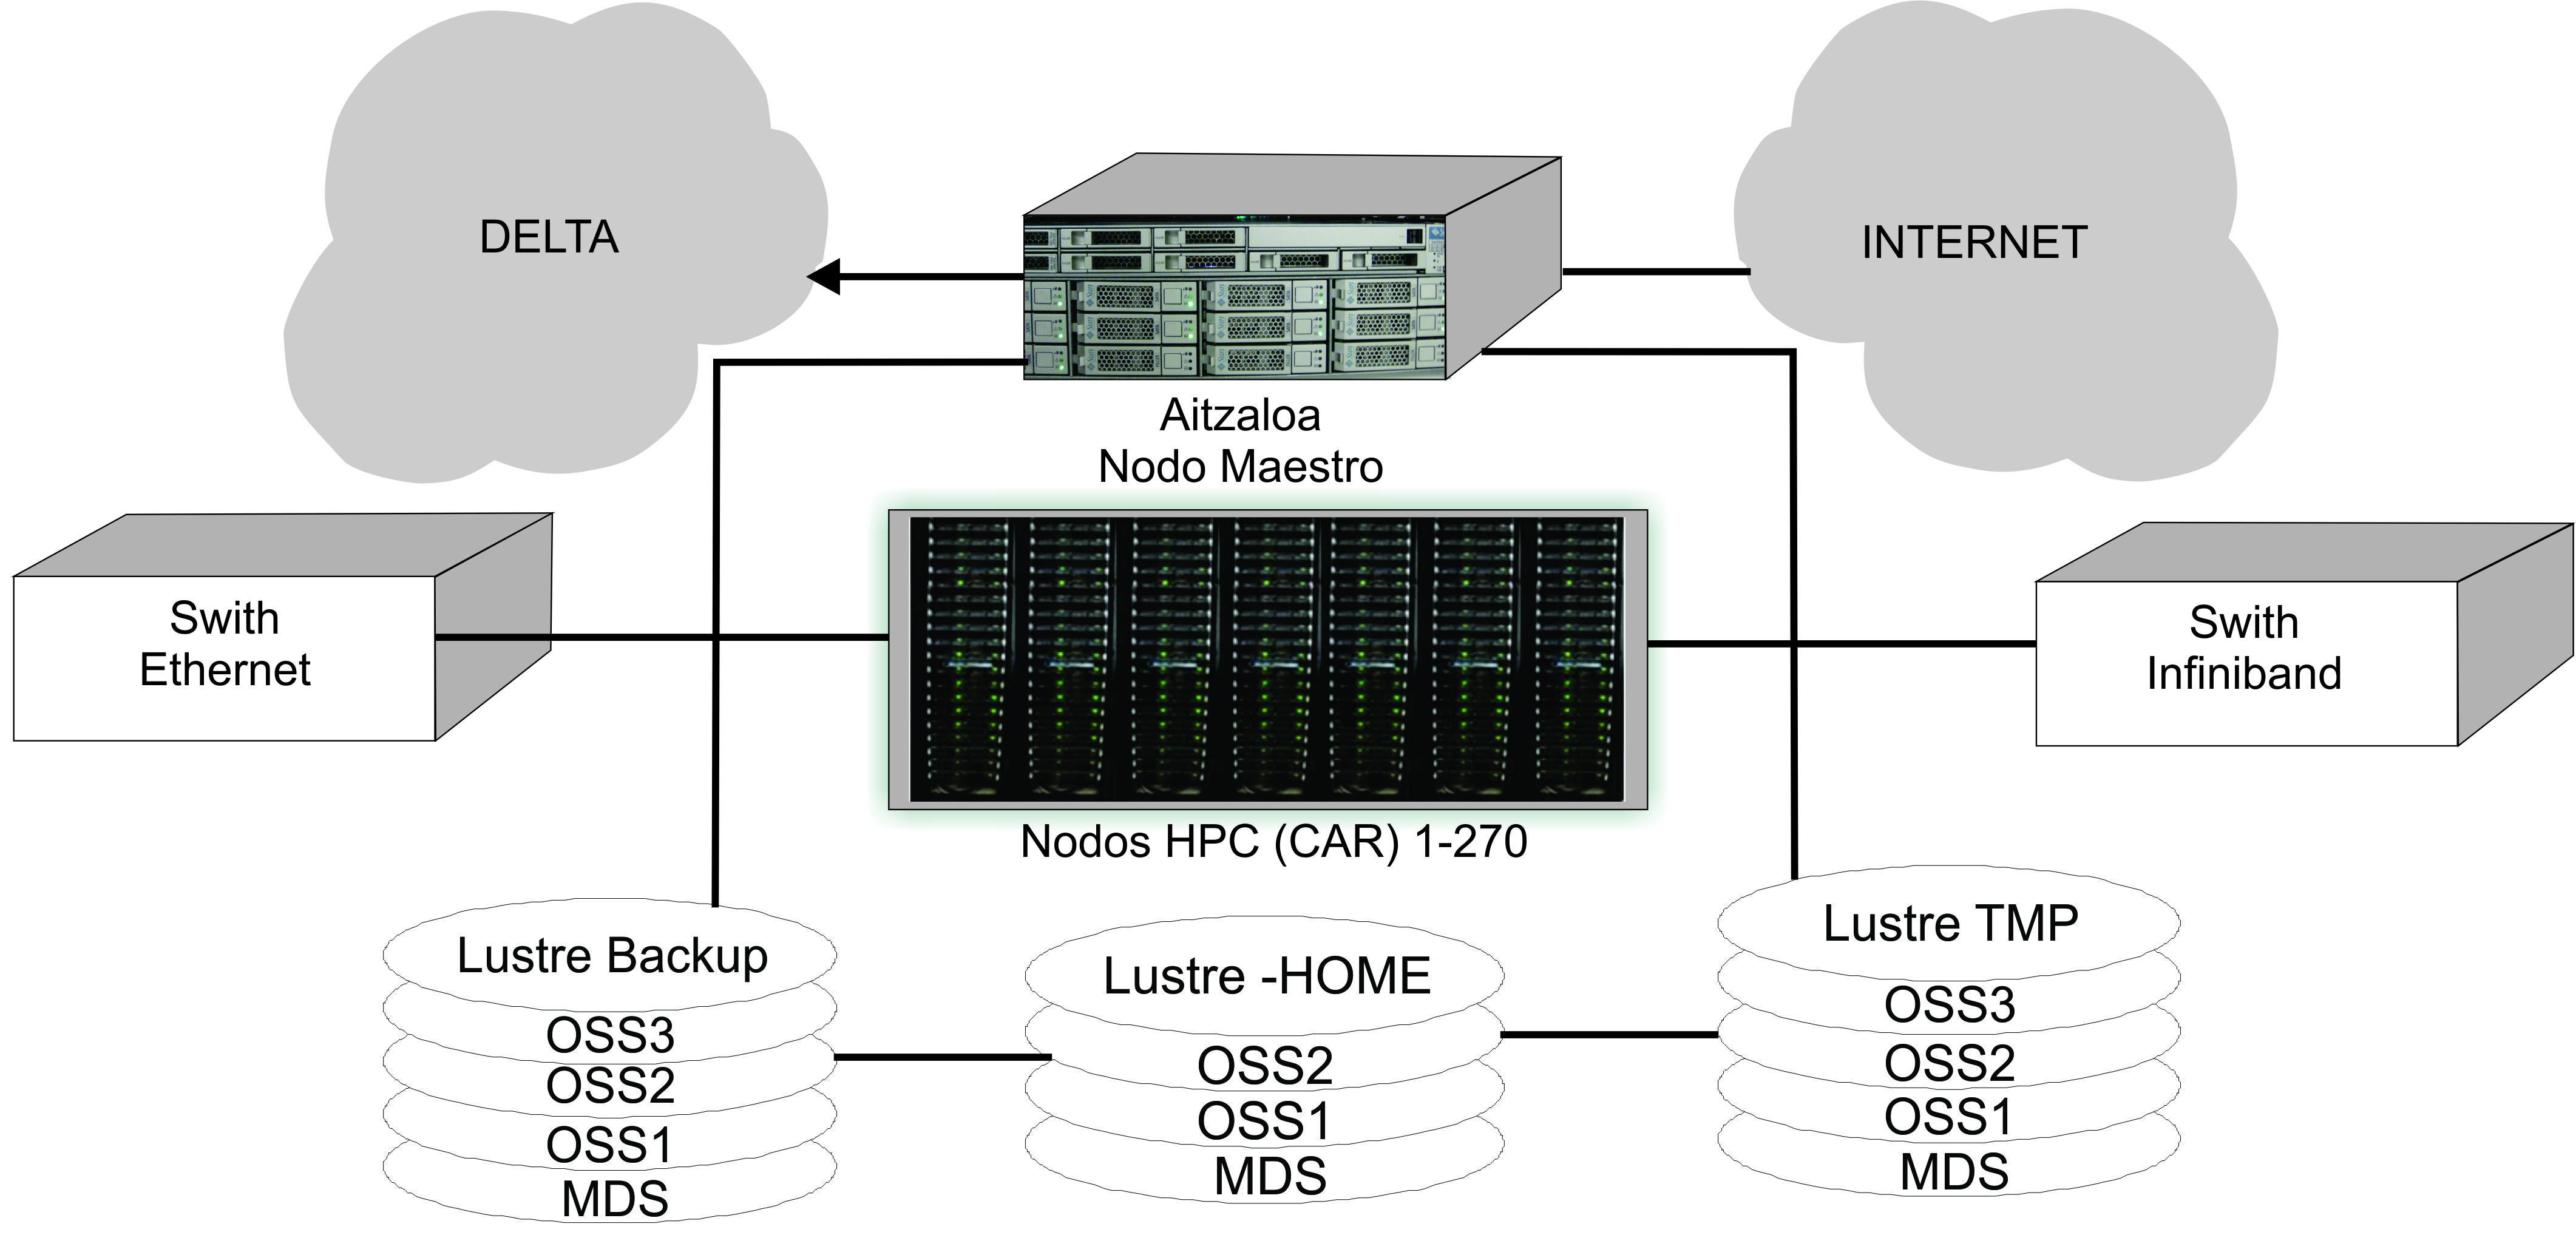
\includegraphics[width=0.8\textwidth]{imagenes/topologia_aitzaloa}
    \end{center}
    \caption{Topología del cluster Aitzaloa}
    \label{fig:topologia_aitzaloa}
\end{figure}


\subsection{Grids}
Los \emph{grids} son sistemas distribuidos, paralelos, compuestos de computadoras autónomas y geográficamente distribuidas que pueden trabajar en conjunto o de manera independiente de acuerdo a los objetivos, políticas y mecanismos de uno o varios administradores del sistema, es decir, un grid puede ser compartido entre varias instituciones \cite{buyya2009cloud}. 

El proyecto \emph{LANCAD}\footnote{Laboratorio Nacional de Cómputo de Alto Rendimiento} es un buen ejemplo, pues une el cluster \emph{Aitzaloa} de la UAM, el cluster de la UNAM \emph{KamBalam}, y el cluster \emph{Xiuhcoatl} del CINVESTAV por medio de una red de fibra óptica instalada en las estaciones del Sistema de Transporte Colectivo Metro. La suma de la potencias reales de cada \emph{nodo robusto} del grid es de 48.55 teraFLOPS \cite{lancad2013xiuhcoatl}.

En la figura \ref{fig:LANCAD-mapa-fo} se muestra los tramos de línea de Metro que cuentan con fibra óptica para conectar cada uno de las supercomputadoras (clusters) de las tres instituciones.

\begin{figure}
    \begin{center}
        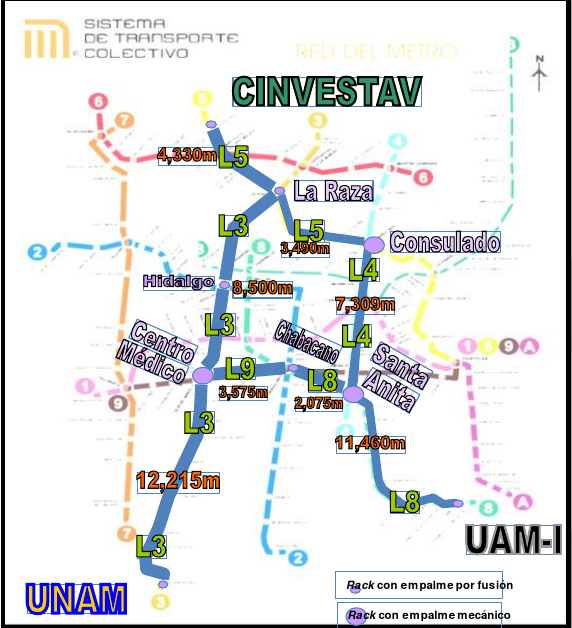
\includegraphics[width=0.8\textwidth]{imagenes/LANCAD-mapa-fo}
    \end{center}
    \caption{Red de fibra óptica del grid LANCAD.}
    %Detalle de la red de fibra óptica para conectar los nodos robustos del grid del proyecto LANCAD
    \label{fig:LANCAD-mapa-fo}
\end{figure}


\subsection{Nubes}
Las \emph{nubes} (clouds) son sistemas distribuidos, paralelos, compuestos de computadoras o máquinas virtuales interconectadas que son aprovisionadas para usarse como uno o varios recursos de cómputo, de acuerdo a un contrato de nivel de servicio acordado entre el proveedor de la nube y el cliente \cite{buyya2009cloud}. 

Empresas nuevas y existentes proveen servicios de cómputo en la nube, tales como GoGrid, Rackspace, Amazon, Microsoft, IBM, Oracle, entre otras. La forma en que operan es la siguiente: se paga cierta cantidad por utilizar servicios de cómputo o almacenamiento durante determinado tiempo. Así, los clientes no tienen que invertir grandes cantidades de dinero para contar con una gran infraestructura como en el caso de los clusters y los grids.

\section{Comparación de los enfoques}
Si bien estos enfoques difieren, principalmente, en la forma en que están organizadas las unidades de cómputo, podemos enumerar algunas observaciones.

Primero, es natural ver que los grids están compuestos de clusters, pero también podría verse a un grid como un gran cluster. Hasta cierto punto este razonamiento parece correcto. Sin embargo, la diferencia importante entre clusters y grids radica en el hecho de que el grid es comúnmente administrado por varios técnicos de varias instituciones que, pueden tener objetivos y necesidades diversas, mientras que un cluster requiere de menos administradores y se asume una mayor flexibilidad para enfrentar fallos. \cite{buyya2009cloud} %Esta comparación viene en la primera tablita del paper%

Segundo, tanto los grids como las nubes son físicamente muy similares: ambos consisten de varios clusters interconectados y distribuidos geográficamente. Entonces, ¿cuál es la diferencia? Lo que distingue a las nubes de los grids son dos características: (1) en una nube, se utilizan \emph{máquinas virtuales} para distribuir el recurso. El usuario tiene la vista de una parte del grid como si fuera una computadora dedicada exclusivamente para éste. Por otro lado, en los grids, es común que el usuario acceda a él con una cuenta asignada por un administrador, de tal suerte que se tiene una vista de una gran máquina que es compartida entre varios usuarios. Muchos de los administradores de grids en el mundo administran los trabajos encargados por los usuarios de tal modo que se ejecuten lo más rápido posible con los recursos disponibles en un tiempo dado. Los usuarios, en algunos casos obtienen acceso al grid y trabajan sus proyectos de manera gratuita o, en caso contrario, pagan una cuota por un tiempo fijo de cómputo. Pero, en el caso de las nubes, se agrega un modelo económico para acceder a los recursos llamado \emph{pay as you go}, en donde el usuario paga una cuota proporcional a los recursos utilizados. Así, el usuario podría pagar una gran cantidad para que su flujo de trabajo se ejecute en el menor tiempo posible o también podría pagar una menor cantidad sacrificando el tiempo total de ejecución del flujo.
\chapter{Planificación}
La planificación
%\footnote{También conocida en la literatura especializada como \emph{scheduling}}
es el proceso de asignación de recursos a tareas, de tal modo que se define un orden de ejecución de las tareas, teniendo lugar diferentes combinaciones de recursos y tareas. En este capítulo se define de la forma más elemental el problema de la planificación para estudiar sus propiedades y también se explica la relación de este problema fundamental con los flujos de trabajo.


\section{Definición del problema}
\label{secc:scheduling_problem}
De acuerdo a  Ullman et al. \cite{ullman1975np}, el problema de la planificación se define de la siguiente manera: 

%al parecer hay que usar la definición extendida de Ullman para que muestre a la planificación como una función f
\begin{defn}
El \textbf{problema de la planificación} está compuesto por:
\begin{enumerate}
\item Un conjunto de tareas $S = \{ J_1, J_2, \dots, J_n \}$
\item Un ordenamiento parcial $\prec$ sobre $S$
\item Una función de costo $U: S \mapsto \mathbb{Z}^{+}$, la cual indica el tiempo que tarda en completarse cada una de las tareas en $S$
\item Un número de computadoras (procesadores) $k$
\end{enumerate}
\end{defn}

Para Ullman et al. \cite{ullman1975np}, el objetivo del problema de la planificación es \emph{minimizar} el tiempo total de ejecución, denotado por $t_\text{max}$, respetando el orden parcial definido por $\prec$, asignando tareas de $S$ a los $k$ procesadores.
También, es importante notar que se asume que cuando una computadora ejecuta una tarea, ésta es ejecutada completamente, sin errores o interrupciones.

\section{La complejidad de planificar}
Como puede notarse, hay varias maneras de acomodar las $k$ computadoras para que se ejecuten todas las tareas de $S$. De hecho, Ullman et al. han demostrado que este problema pertenece a la categoría NP-completo \cite{ullman1975np}. Esto signifca que no se ha encontrado un algoritmo que pueda resolver el problema en tiempo polinomial. Entonces, la solución ingenua de probar ordenadamente todas las posibles asignaciones de tareas a computadoras resulta computacionalmente muy costoso.

Así, la forma de atacar estos problemas NP-completos es utilizar métodos de aproximación \cite{leiserson2001introduction} que obtengan soluciones subóptimas o utilizar heurísticas que resuelvan este problema asumiendo ciertas restricciones.

\section{Planificación de flujos de trabajo}
Hasta ahora, se ha mencionado el problema básico de planificación con restricciones. Con ello, se pretende plantear el problema de la planificación de flujos de trabajo y apoyarse en la definición del problema básico de planificación para enumerar propiedades sobre este problema.

Para plantear el problema de la planificación de flujos de trabajo, primero se mostrará que, bajo ciertas condiciones, un flujo de trabajo puede ser reducido a un grafo dirigido acíclico haciendo las transformaciones adecuadas. Luego, se utilizará la definición del problema básico de planificación con restricciones y su semejanza para flujos de trabajo. Finalmente, se hará una descripción de la complejidad de planificar flujos de trabajo.
%tres hechos:
% - todo flujo de trabajo puede reducirse a DAG
% - transforma un DAG a un problema clásico de Ullman
% - menciona que el problema de Ullman es NP-completo
\subsection{Reducción de flujos de trabajo a grafos dirigidos acíclicos}
En el trabajo de Mair et al. \cite{mair2007workflow} se propone un formato para una representación intermedia de flujos de trabajo basada en grafos dirigidos acíclicos, con el fin de transformar una especificación detallada de un flujo de trabajo, escrita en un lenguaje basado en XML llamado AGWL, a esta representación intermedia. Como se vio en el capítulo \ref{chap:workflows}, un flujo de trabajo puede ser interpretado desde varias perspectivas. Sin embargo, un grafo dirigido acíclico resume en pocos elementos (nodos y aristas), las tareas y las dependencias que deben ser cumplidas durante la planificación. Es por esta razón que es deseable reducir un flujo de trabajo, interpretado desde cualquier perspectiva, a un grafo dirigido acíclico.

%reflejada en las distintas formas de representación que los sistemas de administración de flujos de trabajo utilizan para operar
Cabe aclarar que, como se vio en el primer capítulo de este trabajo, aún no existe un conseso sobre qué representa un flujo de trabajo \cite{van2003workflow}, debido a las diferentes perpectivas de interpretación de un flujo. En el caso del lenguaje AGWL, éste cuenta con facilidades para poder expresar flujos de trabajo condicionales, a saber: constucciones if, while, for y parallel. Estas facilidades permiten expresar una gran variedad de flujos de trabajo. Sin embargo, para poder estudiar los flujos de trabajo con estas construcciones, se requieren de mecanismos de predicción o estimación de posibles rutas de ejecución del flujo de trabajo. En algunos sistemas de administración de ejecución de flujos de trabajo, como Pegasus \cite{deelman2005pegasus}, aplican desenroscado de bucles como técnica de estimación de la ruta de ejecución del flujo, para transformar el flujo de trabajo condicional en un grafo dirigido acíclico. Sin embargo, el estudio de estos mecanismos está fuera del alcance de este trabajo.

%Aunque no existe un consenso general sobre cuál es una definición completa de un flujo de trabajo \cite{van2003workflow}, el lenguaje AGWL es una especificación suficientemente flexible para expresar una gran cantidad de flujos de trabajo, porque con las construcciones if, while, for, parallel, secuence son adecuadas para expresar vastos flujos.

%El hecho importante a recalcar es que los grafos dirigidos acíclicos sirven como representación para utilizarlos en los algoritmos de planificación.

De esta forma, es posible asumir, tanto para el estudio del problema de planificación de flujos de trabajo como para los algoritmos de planificación, que se tendrá como entrada la representación del flujo de trabajo en forma de un grafo dirigido acícliclo.

\subsection{Definición del problema de planificación de flujos de trabajo}
Una vez que se ha establecido a los grafos dirigidos acíclicos como nuestra representación básica de flujos de trabajo, se definirá el problema que conlleva asignar recursos a las tareas del flujo.

Con el fin de no perder generalidad, tomaremos la definiciones de Wieczorek-Prodan \cite{wieczorek2008taxonomies} para definir el problema de la planificación de flujos de trabajo:

\begin{defn}
Un \textbf{flujo de trabajo} es un grafo dirigido $w \in \mathcal{W}, w = (\mathcal{V},\mathcal{E})$, compuesto de un conjunto de nodos $\mathcal{V}$ que representan tareas $ \tau \in \mathcal{T}$ y un conjunto de aristas $\mathcal{E}$ que representan transferencias de datos $ \rho \in \mathcal{D}$.
\end{defn}

Hay que notar que en la definición anterior que la forma en que se relacionan las tareas y las transferencias de datos con los nodos y aristas del grafo está determinada por la representación del flujo de trabajo.
%\emph{concreta}
%creo que esto requiere más trabajo.

Ahora, se definirán los recursos de cómputo en donde se ejecuta el flujo. 
%La definición de Wieczorek-Prodan habla de grids, pero es fácilmente aplicable a otros enfoques de cómputo.

\begin{defn}
Un \textbf{servicio} es una entidad de cómputo que puede ejecutar una tarea $\tau \in \mathcal{T}$. El conjunto de todos los servicios disponibles para ejecutar el flujo de trabajo está denotado por $\mathcal{S}$.
\end{defn}

De este modo, la planificación es definida como una función:

\begin{defn}
La \textbf{planificación de un flujo de trabajo} $w$ es una función $ f: \mathcal{T} \mapsto \mathcal{S}$ que asigna servicios a las tareas del flujo. El conjunto que contiene todas las posibles calendarizaciones de $w$ es denotado por $\mathcal{F}$.
\end{defn}

Cada posible planificación determina un costo de ejecución. A continuación, definiremos el modelo de costo determinado por la utlización de los servicios.

\begin{defn}
Un \textbf{modelo de costos} es un conjunto de criterios $C = \{c_1, c_2, \dots, c_n\}$ que determinan las restricciones en las que se debe ejecutar una planificación, por ejemplo, un límite en el tiempo de ejecución, en el costo monetario o la tolerancia a fallos, entre otros.
\end{defn}

\begin{defn}
Para cada criterio $c_i \in C$, existe una \textbf{función de costo parcial} $\Theta_i : \mathcal{S} \mapsto \mathbb{R}$, en la que a cada servicio disponible para ejecutar el flujo de trabajo se le asocia un costo por ejecutar dicho servicio con las restricciones dictadas con el criterio $c_i$.
\end{defn}

\begin{defn}
Para cada criterio $c_i \in C$, existe una \textbf{función de costo total} $\Delta_i : \mathcal{W} \times \mathcal{F} \mapsto \mathbb{R}$, que asigna un flujo de trabajo $w$ calendarizado por $f$ un costo basado en los costos parciales determinados por los servicios utlizados para ejecutar las tareas del flujo.
\end{defn}

El objetivo del problema de la planificación de flujos de trabajo es encontrar la planificación $f$ que minimice las funciones de costo total $\Delta_i$, $1 \le i \le n$.

\subsection{Complejidad computacional de la planificación de flujos de trabajo}
%Después de haber enunciado varias definiciones para definir el problema de la planificación de flujos de trabajo
Ahora, se hará una analogía con el problema básico de planificación visto en la sección \ref{secc:scheduling_problem} para estudiar su complejidad computacional. La analogía es la siguiente:


\begin{enumerate}
\item El conjunto de tareas $S$ equivale a las tareas $\mathcal{T}$ descritas por el flujo de trabajo.

\item El ordenamiento parcial $\prec$ está representado tanto por las dependencias de datos $\mathcal{D}$ y las aristas $\mathcal{E}$ que representan el control de flujo que debe respetarse para ejecutar el flujo.

\item Las $k$ computadoras equivalen al conjunto de servicios $\mathcal{S}$ disponibles para ejecutar el flujo.

\item La función de costo $U$ tiene una equivalencia implícita. El problema básico asume que conocemos apriori el tiempo de ejecución de una tarea. Sin embargo, es muy frecuente que sólo tengamos una estimación del tiempo de ejecución. Por otro lado, podemos establecer una función auxiliar que relacione las tareas con los servicios. Dicha relación es la función de planificación $f$. En efecto, ejecutar una tarea en un servicio genera un costo, determinado por las funciones parciales y totales. Por lo pronto, estableceremos una relación proporcional entre costo y tiempo, con el fin de mostrar que existe una equivalencia entre la función de costo $W$ del problema básico y el modelo de costo de un flujo de trabajo.
\end{enumerate}

Con lo anterior, se ha mostrado que el problema de la planificación de flujos de trabajo es equivalente al problema básico de planificación. Entonces, se puede inferir que el problema de la planificación de flujos de trabajo pertenece a la categoría de problemas NP-completo.

%tareas -> servicios -> costo <=> tiempo
\chapter{Algoritmos de calendarización de flujos de trabajo}
En el capítulo anterior definimos el problema de calendarizar flujos de trabajo. También se vio que dicho problema pertenece a la categoría de los problemas NP-completos, lo cual significa que la complejidad --o tiempo de ejecución-- para resolver este problema no está acotada por una función polinomial. Por ello, diversos algoritmos se han propuesto para atacar, ya sea de manera total o parcial, el objetivo principal de la calendarización: optimizar el tiempo de ejecución total.

Ahora, con los enfoques de cómputo propuestos en el capítulo 2, se crean diversos algoritmos para diferentes necesidades. Mientras que en los clusters y los grids se asumen que estos recursos son compartidos, los algoritmos de calendarización para estos recursos asumen que los flujos deben ser ejecutados lo más pronto posible, con el fin de hacer que el recurso esté ocupado la mayor parte del tiempo. Por otro lado, el enfoque de nubes permite diseñador de flujos de trabajo elegir entre ejecutar el flujo con todos los recursos a costa de un elevado presupuesto o, minimizar dicho presupuesto tolerando un tiempo de ejecución mayor al mínimo posible.

De acuerdo a Yu et al. \cite{yu2008workflow}, se pueden clasificar los algoritmos de calendarización los algoritmos de flujos de trabajo ejecutados en grids en dos grandes niveles: los algoritmos de Mejor Eesfuerzo y los algoritmos de Calidad en el Servicio\footnote{En la literatura especializada se conoce a este término como \emph{Quality of Service}}. Al primer grupo pertenecen aquellos algoritmos que tratan de minimizar el tiempo total de ejecución\footnote{También conocido como \emph{makespan}}, haciendo uso de todos los recursos disponibles. El segundo grupo, los algoritmos tratan de obtener una calendarización que cumpla las restricciones especificadas como una medida de calidad, con la posibilidad de elegir soluciones que tomen un tiempo de ejecución subóptimo.

A continuación, mostraremos los algoritmos descritos en el trabajo de Yu et al., con los ajustes en notación necesarios para que coincidan con las definiciones de flujo de trabajo establecidas en el capítulo anterior.


\section{Algoritmos de Mejor Esfuerzo}
Este tipo de algoritmos tratan de minimizar algún criterio, que en muchos casos es el tiempo total de ejecución o \emph{makespan}. Cabe aclarar que para los siguientes algoritmos, se asumirá que el grafo del flujo de trabajo tiene una correspondencia biyectiva entre los nodos $mathcal{V}$ y las tareas $mathcal{T}$, es decir, cada nodo del grafo representa una tarea del flujo de trabajo. Las aristas del grafo representan \emph{dependencias entre tareas}.

\subsection{Myopic (miope)}
Este es el más simple de todos los algoritmos. Lo único que hace es buscar un recurso disponible que pueda ejecutar la tarea y asignarle dicha tarea. No toma en cuenta otra característica a optimizar. Este algoritmo fue propuesto por Ramamritham et al. \cite{ramamritham1990efficient}. Ell algoritmo \cite{yu2008workflow} peresentado en estre trabajo se encuentra en la sección \cite{alg:myopic} del Apéndice.

\subsection{Min-min}
El algoritmo min-min está basado en la heurística de terminar las tareas más cortas en el menor tiempo posible. Para ello, hace una estimación del tiempo de ejecución tomando en cuenta el tiempo de preparación de las tareas en los servicios --o recursos-- para tener el tiempo y los archivos necesarios disponibles para el recurso en cuestión. El algoritmo fue presentado por Maheswaran et al. \cite{maheswaran1999dynamic}. El pseudocódigo está descrito en el listado \ref{alg:min-min}.

\subsection{Max-min}
El algoritmo max-min --también propuesto Maheswaran et al. \cite{maheswaran1999dynamic}-- es muy similar al algoritmo min-min. La diferencia radica en que éste calendariza tareas cuyo tiempo mínimo de ejecución es el mayor, de tal modo que se ejecutan las tares más \emph{largas}.

El único cambio que se necesita hacer al algoritmo \ref{alg:min-min} es cambiar la siguiente línea (14):
\[T \leftarrow \arg\min_{t \in \emph{availTasks}}ECT(t,r);\]
por
\[T \leftarrow \arg\max_{t \in \emph{availTasks}}ECT(t,r);\]
Así, el algoritmo modificado puede verse en el pseudocódigo \ref{alg:max-min}.

\subsection{Sufragio}
El algoritmo Sufragio\footnote{También conocido como \emph{Sufferage}} \cite{maheswaran1999dynamic} es una variación del algoritmo Min-min, el cual considera el valor del sufragio para hacer la calendarización. Dicho valor es la diferencia entre el menor tiempo de ejecución para una tarea $t$ sobre un conjunto de recursos disponibles y el segundo menor. Se calendariza a la tarea que tenga el valor del sufragio más alto, por el hecho de que las tareas que son muy sensibles a los cambios de los recursos deben ser calendarizadas primero. El algoritmo se encuentra en la sección \ref{alg:sufferage} del Apéndice.



\section{Algoritmos de Calidad en el Servicio}

\section{Problemas adicionales}

\subsection{Estimación del tiempo}
\subsection{Descomposición de tareas}

\chapter[Software para flujos de trabajo]{Software para la administración y ejecución de flujos de trabajo}

En el capítulo anterior se extendió la clasificación de algoritmos de planificación elaborada por Yu et al. \cite{yu2008workflow}. Sin duda, estos algoritmos han sido probados en simulaciones e implementados en sistemas que administran la ejecución de los flujos de trabajo. De acuerdo a Yu el al. \cite{yu2008workflow}, un sistema de administración de flujos de trabajo\footnote{En la literatura académica, estos sistemas son conocidos como \emph{workflow management sofware systems}} se encarga de definir, coordinar y ejecutar los flujos de trabajo en los recursos de cómputo.

Para este trabajo, clasificaremos los sistemas de administración de flujos de trabajo de acuerdo a su enfoque de cómputo, enumerando las siguientes características: año de aparición, proyecto, utilización, autores y los algoritmos de planificación utilizados en estos sistemas.

\section{Software orientado a clusters}

%\subsection{Open Grid Scheduler}
%NO entra!!!, no trabaja con flujos de trabajo o si?

\subsection{HTCondor}
%URL: \url{http://research.cs.wisc.edu/htcondor/}

HTCondor \cite{condor-practice} es un sistema para administrar flujos de trabajo que necesitan ser ejecutados en entornos de cómputo distribuido. Desde 1983 \cite{htcondor2014webpage}, HTCondor es desarrollado y mantenido por la Universidad de Wisconsin en Madison. Éste tiene un módulo llamado DAGman que se encarga de planificar tareas de un flujo de trabajo, expresadas como grafos dirigidos acíclicos. El algoritmo de planificación utilizado por DAGMan es el algoritmo Miope. 

HTCondor presenta al usuario un único recurso de cómputo, formado de varias computadoras interconectadas entre sí. Esta es la razón por la que este sistema de administración de flujos de trabajo cae dentro de la clasificación de software orientado a clusters.

\section{Software orientado a grids}

\subsection{SwinDew-G}
%URL: \url{http://www.swinflow.org/swindew/grid/}

%URL: \url{http://link.springer.com/chapter/10.1007%2F978-1-4614-1933-4_5}

SwinDew-G \cite{yang2007peer} es un sistema de administración de flujos de trabajo cuya característica especial es que trabaja con redes de computadoras P2P. En la primera versión de SwinDew, el proceso de planificación es estático \cite{yang2007peer}, i.e., en la fase de preparación de la ejecución se crea el plan de ejecución del flujo y se aplica sin ninguna modificación a lo largo del tiempo. Varios esfuerzos se han hecho para mejorar el mecanismo de planificación, como el algoritmo CTC \cite{liu2010compromised} diseñado especialmente para flujos de trabajo que son intensivos en instancias pero que contienen pocas tareas simples, como los flujos de trabajo utilizados en los bancos y empresas \cite{liu2011novel}.

%También, existen versiones específicas de SwinDew para nubes. En este caso, citamos la versión para grids llamada SwinDew-G. La primera versión de SwinDew-G aparece en publicaciones aceptadas en el 2006.
Finalmente, SwinDew y sus variantes fueron desarrollados en la Universidad de Swinburne, en Australia.

\subsection{Pegasus}
%URL: \url{https://pegasus.isi.edu/}

Pegasus \cite{deelman2005pegasus} fue desarrollado en la Universidad del Sur de California. Al igual que SwinDew-G, se puede utilizar Pegasus para trabajar con grids y con nubes. Pegassus implementa MaxMin, MinMin y Sufragio como algoritmos de planificación. Las principales aplicaciones de Pegasus son los flujos de trabajo científicos. Los primeros trabajos publicados que reportan el uso de Pegasus datan del 2003 \cite{pegasus2014publications}. Dentro de la arquitectura de Pegasus, el módulo encargado de planificar el flujo de trabajo es el Mapper.

\section{Software orientado a nubes}

\subsection{SwinDew-C}

SwinDew-C \cite{liu2010swindew} es un sistema de administración de flujos de trabajo basado en SwinDew-G, cuya principal característica es que agrega nubes externas como recursos disponibles para la ejecución de flujos de trabajo. La arquitectura de SwinDew-C es muy similar a la arquitectura de SwinDew-G, con la diferencia de que agrega nuevos componentes para manejar restricciones de calidad de servicio y administración de fallos. En el caso de una falla en la ejecución de las tareas, SwinDew-C replanifica la ejecución de la tarea fallida con un algoritmo basado en optimización por colonia de hormigas.
%checar referencia en el paper de SwinDew-C para colonia de hormigas

\subsection{Aneka}
%URL: \url{http://www.manjrasoft.com/products.html}

Aneka \cite{chu2007aneka} es una implementación de una plataforma como servicio que, además de poder especificar y ejecutar flujos de trabajo, también puede planificar y ejecutar aplicaciones distribuidas que hayan sido construidas con distintos modelos de programación distribuida: basado en tareas, basado en threads y basado en MapReduce. El modelo de programación que se utiliza en Aneka para trabajar con flujos de trabajo es el modelo basado en tareas.
%En el primer paper, de grids, se usan estos modelos: task farming y dataflow model.

El diseño de Aneka es basado en servicios. Cada servicio se encarga de una funcionalidad específica para la administración del grid o nube. Así, existe un módulo específico para la planificación de la ejecución de las aplicaciones que varía de acuerdo al modelo de programación elegido para desarrollar la aplicación.

Técnicamente, es posible construir una nube con Aneka \cite{vecchiola2009aneka} utilizando computadoras de escritorio convencionales. De esta forma, Aneka provee servicios para administrar el esquema de precios de la nube construida con este software. Del mismo modo, Aneka utiliza un mecanismo de negociación mediante agentes que buscan \emph{cerrar} los mejores tratos con los proveedores de los servicios de la nube, que mejor satisfagan los requisitos de calidad en el servicio.

Es importante mencionar que la plataforma Aneka fue desarrollada inicialmente por el laboratorio GRIDS de la Universidad de Swinburne, en Austraila. Actualmente, Aneka es desarrollado por la empresa Manjrasoft \cite{aneka2014webpage}.

\subsection{Askalon}
%URL: \url{http://www.dps.uibk.ac.at/projects/askalon/}

Askalon \cite{fahringer2005askalon} es un entorno que facilita el desarrollo y la ejecución de flujos de trabajo. Askalon utiliza un lenguaje llamado AGWL para especificar flujos de trabajo. Al igual que Aneka, el diseño de Askalon está basado en servicios, tales como: el motor de promulgación, el administrador de recursos, la base de datos de checkpoints y el planificador.

En el servicio planificador, Askalon utiliza varios algoritmos de planificación: HEFT, Miope y un algoritmo genético. Esto es porque antes de ejecutar el flujo de trabajo, se hace una predicción del tiempo estimado de ejecución de cada tarea. Entonces, hay un módulo encargado de actualizar la información de las predicciones y, en base al resultado de los tres algoritmos, se elige la planificación que mejor cumpla con los requisitos de calidad en el servicio dictados por el usuario.

Actualmente, el proyecto Askalon es desarrollado por la Universidad de Innsbruck, en Austria \cite{askalon2014webpage}.
\chapter{Conclusiones}

%np-completo: no hay solución polinomial
%no hay un scheduler que pueda cambiar entre algoritmos de calendarización
%es muy difícil hacer un modelo general
%stocastic based approach no son estudiados, pero debería verlos



\appendix
%\include{app01-pseudocodes}
\chapter[Pseudocódigos]{Pseudocódigos de algoritmos de planificación de flujos de trabajo}

\section{Algoritmos de mejor esfuerzo}

\subsection{Miope}
El algoritmo miope \cite{yu2008workflow} es el más simple de todos los algoritmos. Lo único que hace es buscar un recurso disponible que pueda ejecutar la tarea y asignarle dicha tarea. No toma en cuenta otra característica a optimizar. Este algoritmo fue propuesto por Ramamritham et al. \cite{ramamritham1990efficient}. 
%El algoritmo peresentado en estre trabajo se encuentra en la sección \ref{alg:myopic} del Apéndice.

\label{alg:myopic}
\begin{algorithmic}[1]
\Require Un grafo de flujo de trabajo $w=(\mathcal{V}, \mathcal{E})$
\Ensure{Una planificación $f$}
\While{$\exists v \in \mathcal{V}$ no completada}
	\State $t \gets$ Obtener una tarea lista, no calendarizada, con padres calendarizados;
	\State $r \gets$ Obtener un recurso que pueda empezar la tarea en el menor tiempo;
	\State Calendarizar $t$ en $r$, i.e., $f(r) = t$;
\EndWhile
\end{algorithmic}

\subsection{Definiciones para los algoritmos Max-Min y Min-min}
\label{alg:def_maxmin}
Los algoritmos min-min y max-min utilizan las siguientes  estimaciones: %definidas en la tabla \ref{tbl:min-min-estimators}. %todo: checar por qué numera RARO
\begin{itemize}
\item{$EET(t,r)$ -- \textbf{Tiempo estimado de ejecución:} Tiempo que el recurso (servicio) $r$ tomará en ejecutar la tarea $t$, desde que la tarea es ejecutada en el recurso}
\item{$EAT(t,r)$ -- \textbf{Tiempo estimado de disponibilidad:} Tiempo en el que el recurso $r$ estará disponible para ejecutar la tarea $t$}
\item{$FAT(t,r)$ -- \textbf{Tiempo de archivo disponible:} Tiempo más pronto en que todos los archivos requeridos por la tarea $t$ están disponibles en el recurso $r$}
\item{$ECT(t,r)$ -- \textbf{Tiempo estimado de terminación:} Tiempo estimado en cual la tarea $t$ terminará su ejecución en el recurso $r$: 
              \[ ECT(t,r) = EET(t,r) + max(EAT(t,r), FAT(t,r)) \]}
\item{$MCT(t)$ -- \textbf{Tiempo mínimo estimado de terminación: } $ECT$ mínimo para la tarea $t$ sobre todos los recursos disponibles, es decir: 
            \[ MCT(t) = \min_{r \in \mathcal{S}} ECT(t,r) \]}
\end{itemize}

\subsection{Min-Min}
El algoritmo min-min está basado en la heurística de terminar las tareas más cortas en el menor tiempo posible. Para ello, hace una estimación del tiempo de ejecución tomando en cuenta el tiempo de preparación de las tareas en los servicios --o recursos-- para tener el tiempo y los archivos necesarios disponibles para el recurso en cuestión. El algoritmo fue propuesto por Maheswaran et al. \cite{maheswaran1999dynamic}. 
%El pseudocódigo está descrito en el listado \ref{alg:min-min}.

\label{alg:min-min}
\begin{algorithmic}[1]
\Require{Un grafo de flujo de trabajo $w=(\mathcal{V}, \mathcal{E})$}
\Ensure{Una planificación $f$}
\While{$\exists v \in \mathcal{V}$ \emph{no completada}}
	\State $t \gets$ Obtener conjunto de tareas listas, no calendarizadas, con padres  calendarizados;
	\State \Call{Planificacion}{$tasks$};
\EndWhile
\Procedure{Planificacion}{$availTasks$}
	\While{$\exists t \in availTasks$ no planificadas}
		\For{$t \in availTasks$}
			\State $res \gets$ Obtener recursos disponibles para $t$;
			\For{$r \in res$}
				\State Calcular $ECT(t,r)$;
			\EndFor
			\State $R_T \gets \arg\min_{r \in res}ECT(t,r)$;
		\EndFor
		\State $T \gets \arg\min_{t \in availTasks}ECT(t,R_T)$;
		\State Planificar $T$ en $R_T$;
		\State Remover $T$ de \emph{availTasks};
		\State Actualizar $EAT(R_T)$;
	\EndWhile
\EndProcedure
\end{algorithmic}

\subsection{Max-Min}
El algoritmo max-min --también propuesto Maheswaran et al. \cite{maheswaran1999dynamic}-- es muy similar al algoritmo min-min. La diferencia radica en que éste calendariza tareas cuyo tiempo mínimo de ejecución es el mayor, de tal modo que se ejecutan las tares más \emph{largas}.

El único cambio que se necesita hacer al algoritmo \ref{alg:min-min} es cambiar la línea 14:
\[T \leftarrow \arg\min_{t \in \emph{availTasks}}ECT(t,r);\]
por
\[T \leftarrow \arg\max_{t \in \emph{availTasks}}ECT(t,r);\]
Así, el algoritmo modificado puede verse a continuación: %en el pseudocódigo \ref{alg:max-min}.

\label{alg:max-min}
\begin{algorithmic}[1]
\Require{Un grafo de flujo de trabajo $w=(\mathcal{V}, \mathcal{E})$}
\Ensure{Una planificación $f$}
\While{$\exists v \in \mathcal{V}$ \emph{no completada}}
	\State $t \gets$ Obtener conjunto de tareas listas, no planificadas, con padres planificados;
	\State \Call{Planificar}{$t$};
\EndWhile
\Procedure{Planificar}{$tareas$}
	\While{$\exists t \in tareas$ no planificadas}
		\For{$t \in tareas$}
			\State $res \gets$ Obtener recursos disponibles para $t$;
			\For{$r \in res$}
				\State Calcular $ECT(t,r)$;
			\EndFor
			\State $R_T \gets \arg\min_{r \in res}ECT(t,r)$;
		\EndFor
		\State $T \gets \arg\max_{t \in availTasks}ECT(t,R_T)$;
		\State Planificar $T$ en $R_T$;
		\State Remover $T$ de \emph{tareas};
		\State Actualizar $EAT(R_T)$;
	\EndWhile
\EndProcedure
\end{algorithmic}

\subsection{Sufragio}
El algoritmo Sufragio\footnote{También conocido como \emph{Sufferage}} \cite{maheswaran1999dynamic} es una variación del algoritmo Min-min, el cual considera el valor del sufragio para hacer la planificación. Dicho valor es la diferencia entre el menor tiempo de ejecución para una tarea $t$ sobre un conjunto de recursos disponibles y el segundo menor. Se calendariza a la tarea que tenga el valor del sufragio más alto, por el hecho de que las tareas que son muy sensibles a los cambios de los recursos deben ser calendarizadas primero. 
%El algoritmo se encuentra en la sección \ref{alg:sufferage} del Apéndice.

\label{alg:sufferage}
\begin{algorithmic}[1]
\Require{Un grafo de flujo de trabajo $w=(\mathcal{V}, \mathcal{E})$}
\Ensure{Una planificación $f$}
\While{$\exists v \in \mathcal{V}$ \emph{no completada}}
	\State $t \gets$ Obtener conjunto de tareas listas, no planificadas, con padres planificados;
	\State \Call{Planificar}{$t$};
\EndWhile
\Procedure{Planificar}{$tareas$}
	\While{$\exists t \in tareas$ no planificadas}
		\For{$t \in tareas$}
			\State $res \gets$ Obtener recursos disponibles para $t$;
			\For{$r \in res$}
				\State Calcular $ECT(t,r)$;
			\EndFor
			\State $R^1_t \gets \arg\min_{r \in res}ECT(t,r)$;
			\State $R^2_t \gets \arg\min_{r \in res, r \ne{R^1_t}}ECT(t,r)$;
			\State $suf_t \gets ECT(t,R^2_t) - ECT(t,R^1_t)$;
		\EndFor
		\State $T \gets \arg\max_{t \in availTasks}suf_t$;
		\State Planificar $T$ en $R^1_T$;
		\State Remover $T$ de \emph{tareas};
		\State Actualizar $EAT(R_T)$;
	\EndWhile
\EndProcedure
\end{algorithmic}

\subsection{HEFT}
El algoritmo HEFT\footnote{Heterogeneous Earliest-Finish Time} fue propuesto por Topcuoglu et al. \cite{topcuoglu2002performance}. Este algoritmo está dividido en dos fases: (1) priorización de tareas y (2) selección de recursos. En la primera fase, para todas las tareas se calcula un valor llamado $Rango_{Asc}$, que es una estimación del costo de ejecutar una tarea. En la segunda fase, se asigna a cada tarea de la lista un recurso disponible que tenga el tiempo de disponibilidad más corto. Este tiempo se refiere al instante en que un recurso tiene todos los datos necesarios para ejecutar la tarea a planificar.


%Este valor se define de la siguiente forma:

%\begin{equation}
%Rango_{Asc}(t) = \overline{Costo_{comp}(t)} + \max_{n_j \in succ(t)}(\overline{Costo_{comm}(t, n_j)} + Rango_{Asc}(n_j))
%\end{equation}

%Tiempo de ejecución promedio por tarea
El algoritmo HEFT utiliza las fórmulas que vamos a describir a continuación:


Sea $time(T_i, r)$ el tiempo de ejecución de la tarea $T_i$ en el recurso $r$ y sea $R_i$ el conjunto de recursos disponibles para ejecutar la tarea $T_i$. El tiempo de ejecución promedio de la tarea $T_i$ está definido como:
\begin{equation}
\label{ecc:heft1}
\overline{\omega_i} = \frac{\sum_{r \in R_i} time(T_i, r)}{|R_i|}
\end{equation}

Sea $time(e_{ij}, r_i, r_j)$ el tiempo de transferencia de datos entre los recursos $r_i$ y $r_j$ que utilizan el canal $e_{ij}$ para transferir los datos. Sea $R_i$ y $R_j$ los conjuntos de recursos disponibles para ejecutar las tareas $T_i$ y $T_j$, respectivamente. El tiempo promedio de transmisión desde $T_i$ hasta $T_j$ está definido por la siguiente ecuación:
\begin{equation}
\label{ecc:heft2}
\overline{c_{ij}} = \frac{ \sum_{r_i \in R_i, r_j \in R_j} {time(e_{ij}, r_i, r_j)} }{|R_i| |R_j|}
\end{equation}

Cabe recordar que en la primera fase del algoritmo HEFT, las tareas son ordenads de acuerdo a una función de rango. Esta función está definida por partes. Para una tarea de salida $T$, es decir, una tarea que no tiene sucesores que dependan de ella, el valor de rango es determinado por:
\begin{equation}
\label{ecc:heft3}
Rango(T) = \overline{\omega_i}
\end{equation}

Para las tareas que no son tareas de  salida, el valor de rango se calcula con la siguiente expresión:
\begin{equation}
\label{ecc:heft4}
Rango(T) = \overline{\omega_i} + \max_{T_j \in succ(T_i)} ( \overline{C_{ij}} + Rango(T_j) )
\end{equation}
donde $succ(T_i)$ es el conjunto de los sucesores inmediatos de la tarea $T_i$.

\label{alg:heft}
\begin{algorithmic}[1]
\Require{Un grafo de flujo de trabajo $w=(\mathcal{V}, \mathcal{E})$}
\Ensure{Una planificación $f$}
\State Calcular \emph{Tiempo de Ejecución Promedio} \ref{ecc:heft1} para cada tarea $v \in \mathcal{V}$;
\State Calcular \emph{Tiempo de Transferencia de Datos Promedio} \ref{ecc:heft2} entre tareas y sus sucesores;
\State Calcular $Rango_{Asc}$ para cada tarea, de acuerdo a \ref{ecc:heft3} y \ref{ecc:heft4};
\State Ordenar las tareas por $Rango_{Asc}$, en orden decreciente en una lista $Q$;
\While{$Q \ne \varnothing$}
	\State $t \gets$ Remover la primera tarea de $Q$;
	\State $r \gets \arg\min_{r_i \in R}EFT(r_i, t)$ usando \emph{planificación basada en inserciones}
	%\For{$r_i \in R$}
	%	\State Calcular $EFT(r_i, t)$ utilizando la política de \emph{planificación basada en inserciones}
	%\EndFor
	%\State $r \gets$ Encontrar un recurso que pueda ejecutar $t$ en el menor $EFT(r, t)$;
	\State Planificar $t$ en $r$;
\EndWhile
\end{algorithmic}

\subsection{Híbrido}
Este algoritmo combina dos heurístas: primero agrupa las tareas que tengan dependencias entre sí, de tal modo que haya un balance entre el número de grupos y el número de recursos disponibles para la ejecución de las tareas agrupadas. Luego, con los grupos listos, se utiliza un algoritmo de planificación batch para asignar a cada grupo un recurso. Este algoritmo/heurística fue propuesto por Sakellariou et al \cite{sakellariou2004hybrid}. El algoritmo híbrido utiliza las definiciones de tiempos promedio y función de rango del algoritmo HEFT.

\label{alg:hybrid}
\begin{algorithmic}[1]
\Require{Un grafo de flujo de trabajo $w=(\mathcal{V}, \mathcal{E})$}
\Ensure{Una planificación $f$}
\State Calcular \emph{Peso} de cada tarea y arista, de acuerdo a \ref{ecc:heft1} y \ref{ecc:heft2};
\State Calcular \emph{Rango} para cada tarea, de acuerdo a \ref{ecc:heft3} y \ref{ecc:heft4};
\State Ordenar las tareas por \emph{Rango}, en orden decreciente en una lista $Q$;
\State $i \gets 0$
\State Crear un grupo $G_i$;
\While{$Q \ne \varnothing$}
	\State $t \gets$ Remover la primera tarea de $Q$;
	\If{$t$ tiene una dependencia con una tarea en $G_i$}
		\State $i \gets i + 1$;
		\State Crear un grupo $G_i$;
	\EndIf
	\State Agregar $t$ a $G_i$;
\EndWhile
\State $j \gets 0$;
\While{$j \le i$}
	\State Planificar tareas en $G_i$ usando un algoritmo \emph{batch};
	\State $j \gets j + 1$;
\EndWhile
\end{algorithmic}

\subsection{TANH}
\label{alg:tanh}
Bajaj et al. \cite{bajaj2004improving} proponen un algoritmo basado en dos heurísticas: en la duplicación de tareas y en el agrupamiento de tareas. La primera heurística se basa en que si dos tareas dependen del resultado de una tarea en común y, estas dos tareas se encuentran en recursos diferentes y con un tiempo muerto previo a la ejecución de estas tareas, entonces, se ejecuta de forma rendundante la tarea común en los dos recursos diferentes, para que las dos tareas puedan continuar su ejecución de manera independiente y no exista un costo de comunicación de datos entre estos dos recursos. La segunda heurística se refiere a que las tareas con dependencias entre sí se deben ejecutar en los mismos recursos, para que los costos de comunicación de datos sean despreciables.

\begin{algorithmic}[1]
\Require{Un grafo de flujo de trabajo $w=(\mathcal{V}, \mathcal{E})$}
\Ensure{Una planificación $f$}
\State Calcular \emph{Parámetros} para cada nodo tarea;
\State Agrupar tareas del flujo de trabajo;
\If{Número de clusters $\ge$ Número de recursos disponibles}
	\State Reducir el Número de clusters al Número de recursos disponibles;
\Else
	\State Ejecutar duplicación de tareas;
\EndIf
\end{algorithmic}

%\section{Algoritmos de Calidad en el Servicio}
%\subsection{BackTracking}

%\subsection{Deadline Distribution}
%\subsection{CTC}
%\subsection{Deadline-MDP}
%\subsection{LOSS/GAIN}

%\section{Metaheurísticos}
%\subsection{Algoritmo Genético}

\subsection{GRASP}
\label{alg:grasp}
El procedimiento de búsqueda aleatoria voraz adaptativa (GRASP por sus siglas en inglés) es una heurística que se utiliza para resolver problemas de optimización combinatoria. De manera voraz, se construyen planificaciones que reduzcan del tiempo de ejecución total evaluando cada uno de los sucesores de una tarea dada. Así, el algoritmo escoge las tareas de manera aleatoria cuya variación en el tiempo no pase de un rango dado. El algoritmo termina hasta que se cumple un criterio de terminación, como un tiempo límite. Este algoritmo fue propuesto por Blythe et al. \cite{blythe2005task}.

\begin{algorithmic}[1]
\Require{Un grafo de flujo de trabajo $w=(\mathcal{V}, \mathcal{E})$}
\Ensure{Una planificación $f$}
\While{Criterio de terminación no satisfactorio}
	\State $plan \gets$ \Call{crearPlanificacion}{$w$};
	\If{$plan$ es mejor que $mejorPlanificacion$}
		\State $mejorPlanificacion \gets plan$;
	\EndIf
\EndWhile
\Procedure{crearPlanificacion}{$flujo$}
	\State $solucion \gets$ \Call{construirSolucion}{$flujo$};
	\State $nSolucion \gets$ \Call{busquedaLocal}{$solucion$};
	\If{$nSolucion$ es mejor que $solucion$}
		\State \textbf{return} $nSolucion$;
	\EndIf
	\State \textbf{return} $solucion$;
\EndProcedure
\Procedure{construirSolucion}{$flujo$}
	\While{planificación no completada}
		\State $T \gets$ Obtener tareas listas sin asignar;
		\State Crear RCL para cada $t \in T$;
		\State $subSolucion \gets$ Seleccionar recurso \emph{aleatoriamente} para cada $t \in T$ de su RCL;
		\State $solucion \gets solucion \cup subSolucion$;
		\State Actualizar información para futuros RCL;
	\EndWhile
	\State \textbf{return} $solucion$;
\EndProcedure
\Procedure{busquedaLocal}{$solucion$}
	\State $nSolucion \gets$ Encontar una solución local óptima;
	\State \textbf{return} $nSolucion$;
\EndProcedure
\end{algorithmic}

%\subsection{Recocido simulado}


% forma rapida de cambiar "Bibliografía" por "Referencias"
%%\renewcommand*{\bibname}{\chapter*{Referencias}}
\bibliographystyle{plain}
\bibliography{propuesta}
%\addbibresource{propuesta.bib}
%\printbibliography

\end{document}
% must see http://www.cns-ipicyt.mx/html/paginas/solicitud-soporte/
